\newpage

\chapter{Figures} \label{appendix_figures}

\begin{figure} [!htb]
    \centering
    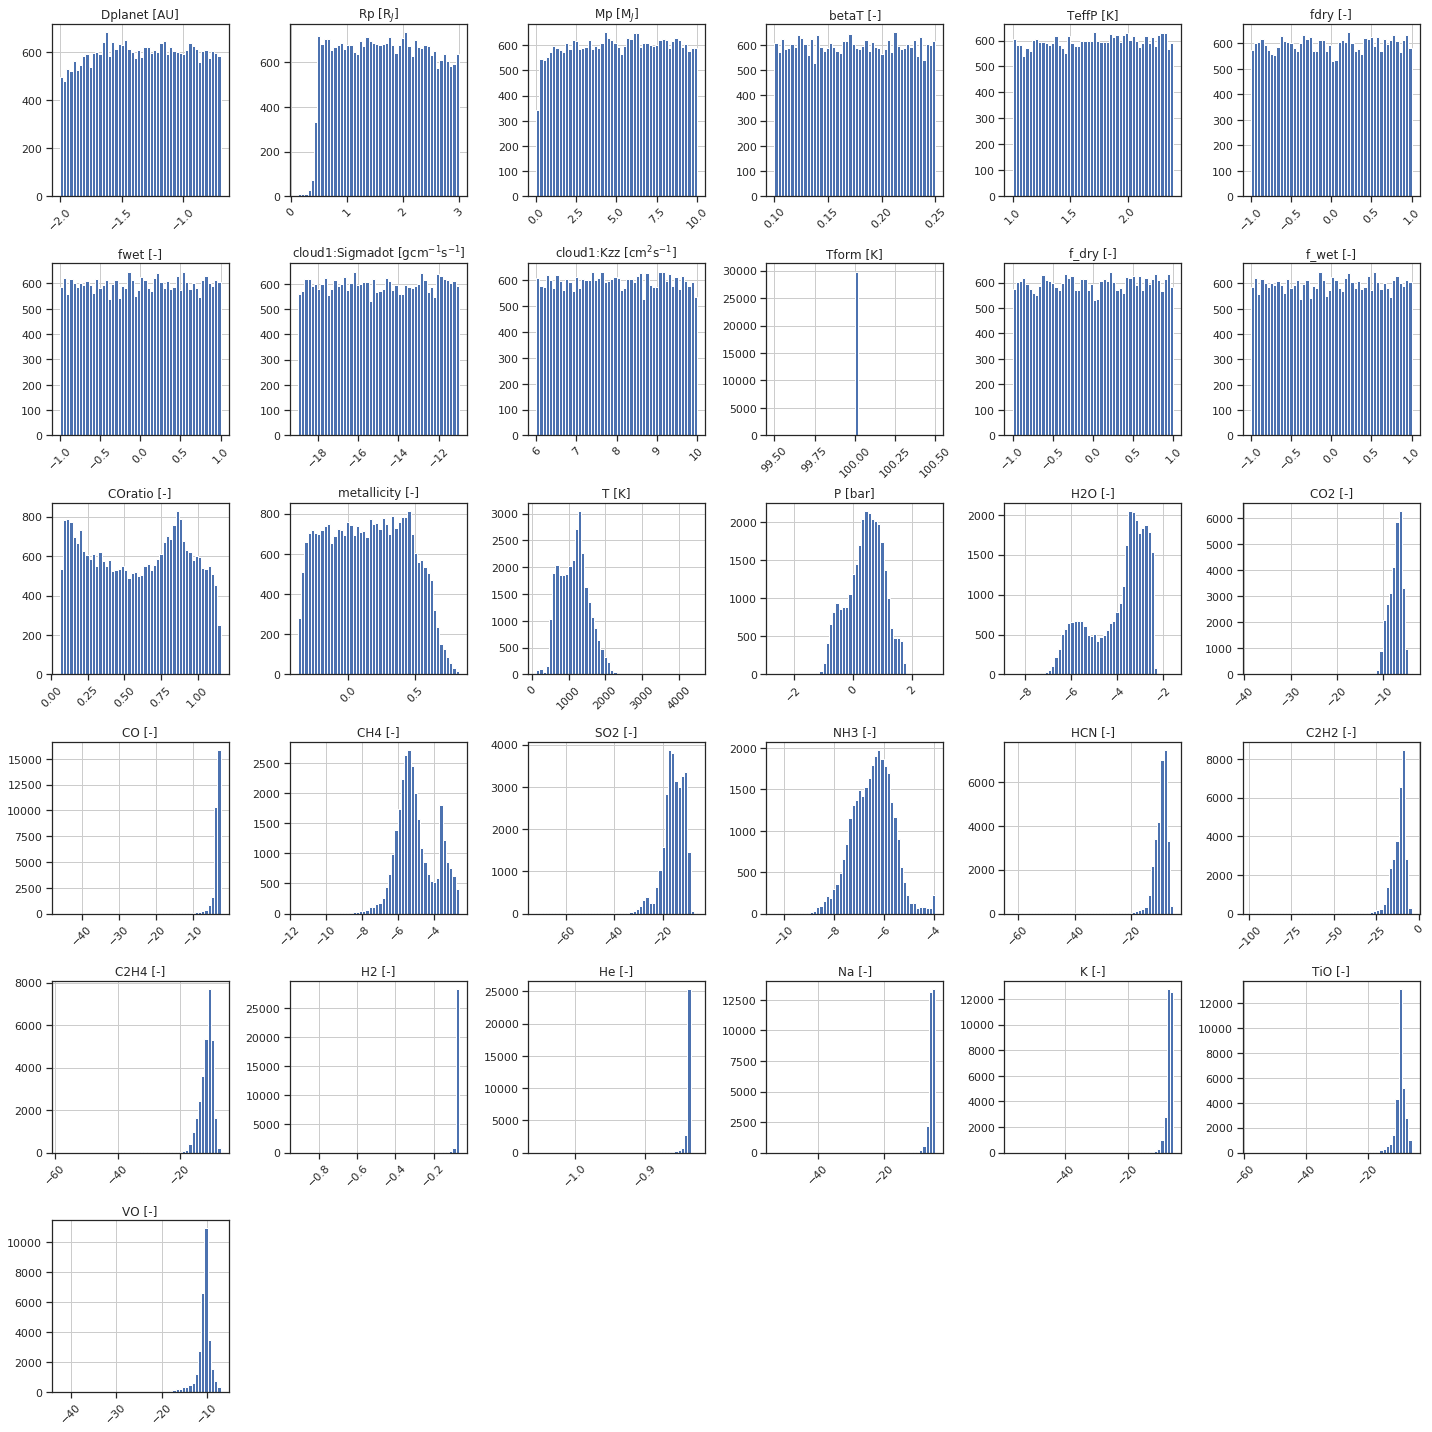
\includegraphics[scale=0.3]{figuren/complex features hist original.png}
    \caption{A data distribution plot containing histograms of all the complex physical features.}
    \label{fig:distribution_original}
\end{figure}

\begin{sidewaysfigure} [!htb]
    \centering
    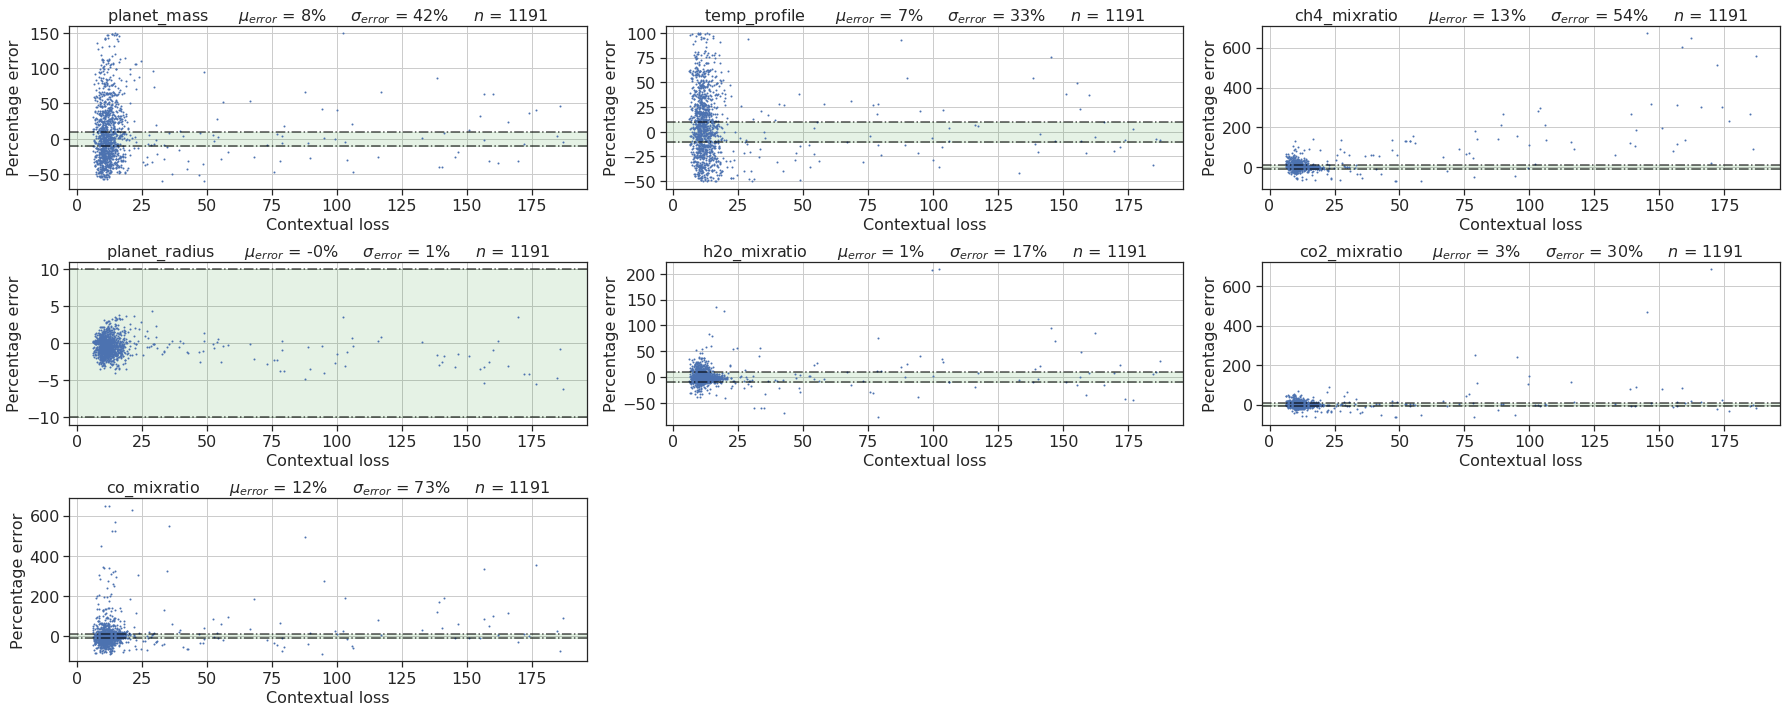
\includegraphics[width=\textwidth,height=\textheight,keepaspectratio]{figuren/contextual errors.png}
    \caption{A visualisation of the error per parameter and its' corresponding contextual loss. Where the green area represent the $\pm$ 10 \% margin.}
    \label{fig:contextual_errors}
\end{sidewaysfigure}

\begin{sidewaysfigure} [!htb]
    \centering
    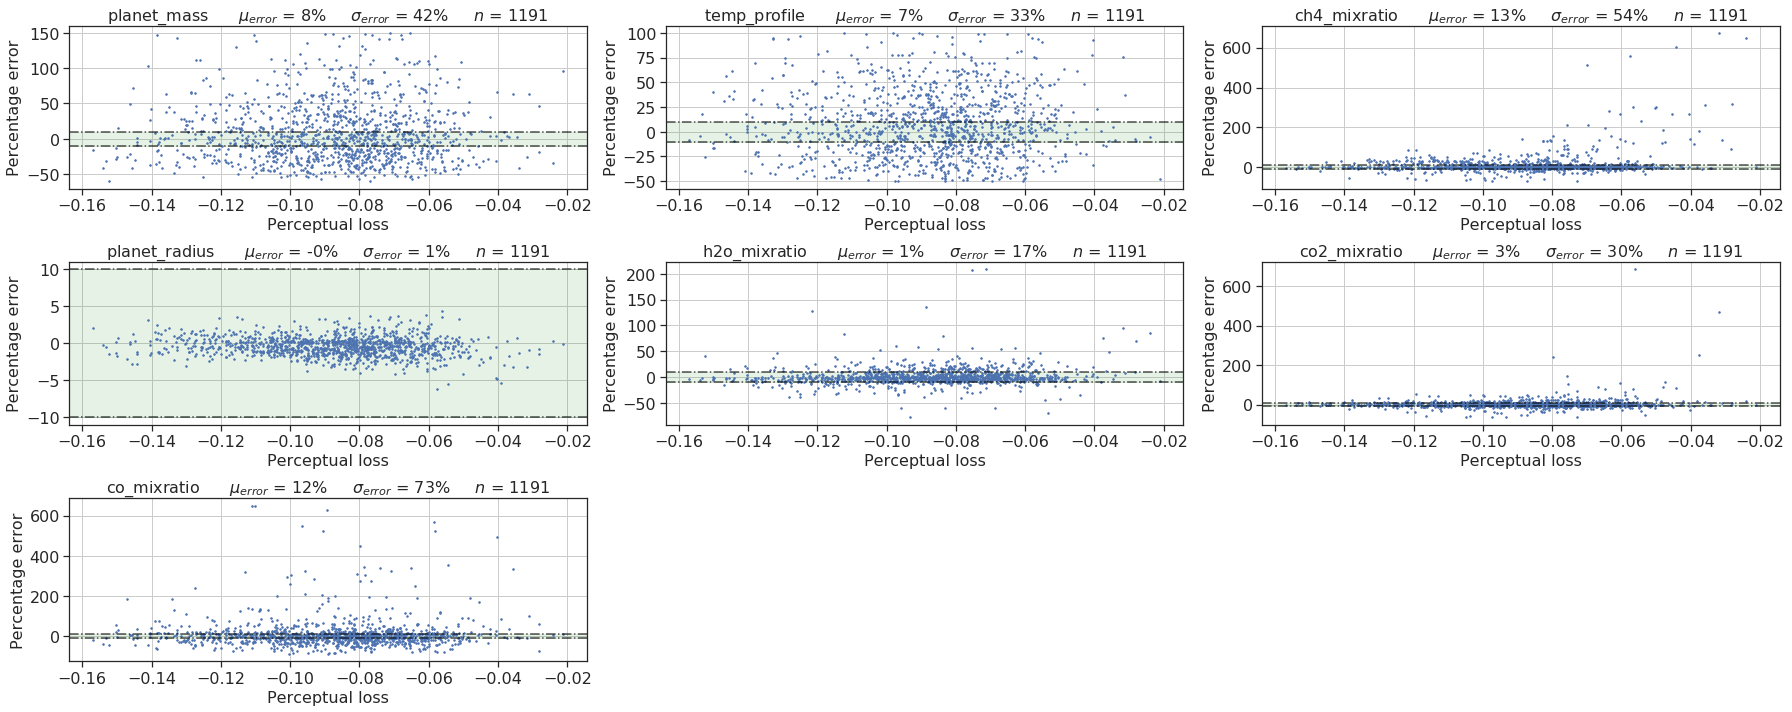
\includegraphics[width=\textwidth,height=\textheight,keepaspectratio]{figuren/perceptual errors.png}
    \caption{A visualisation of the error per parameter and its' corresponding contextual loss. Where the green area represent the $\pm$ 10 \% margin. (in deze plots is te zien dat het inpainten redelijk prima verloopt, maar dat de errors hoog zijn doordat de gan nog niet goed is geconvergeerd).}
    \label{fig:perceptual_errors}
\end{sidewaysfigure}






\begin{figure} [!htb]
    \centering
    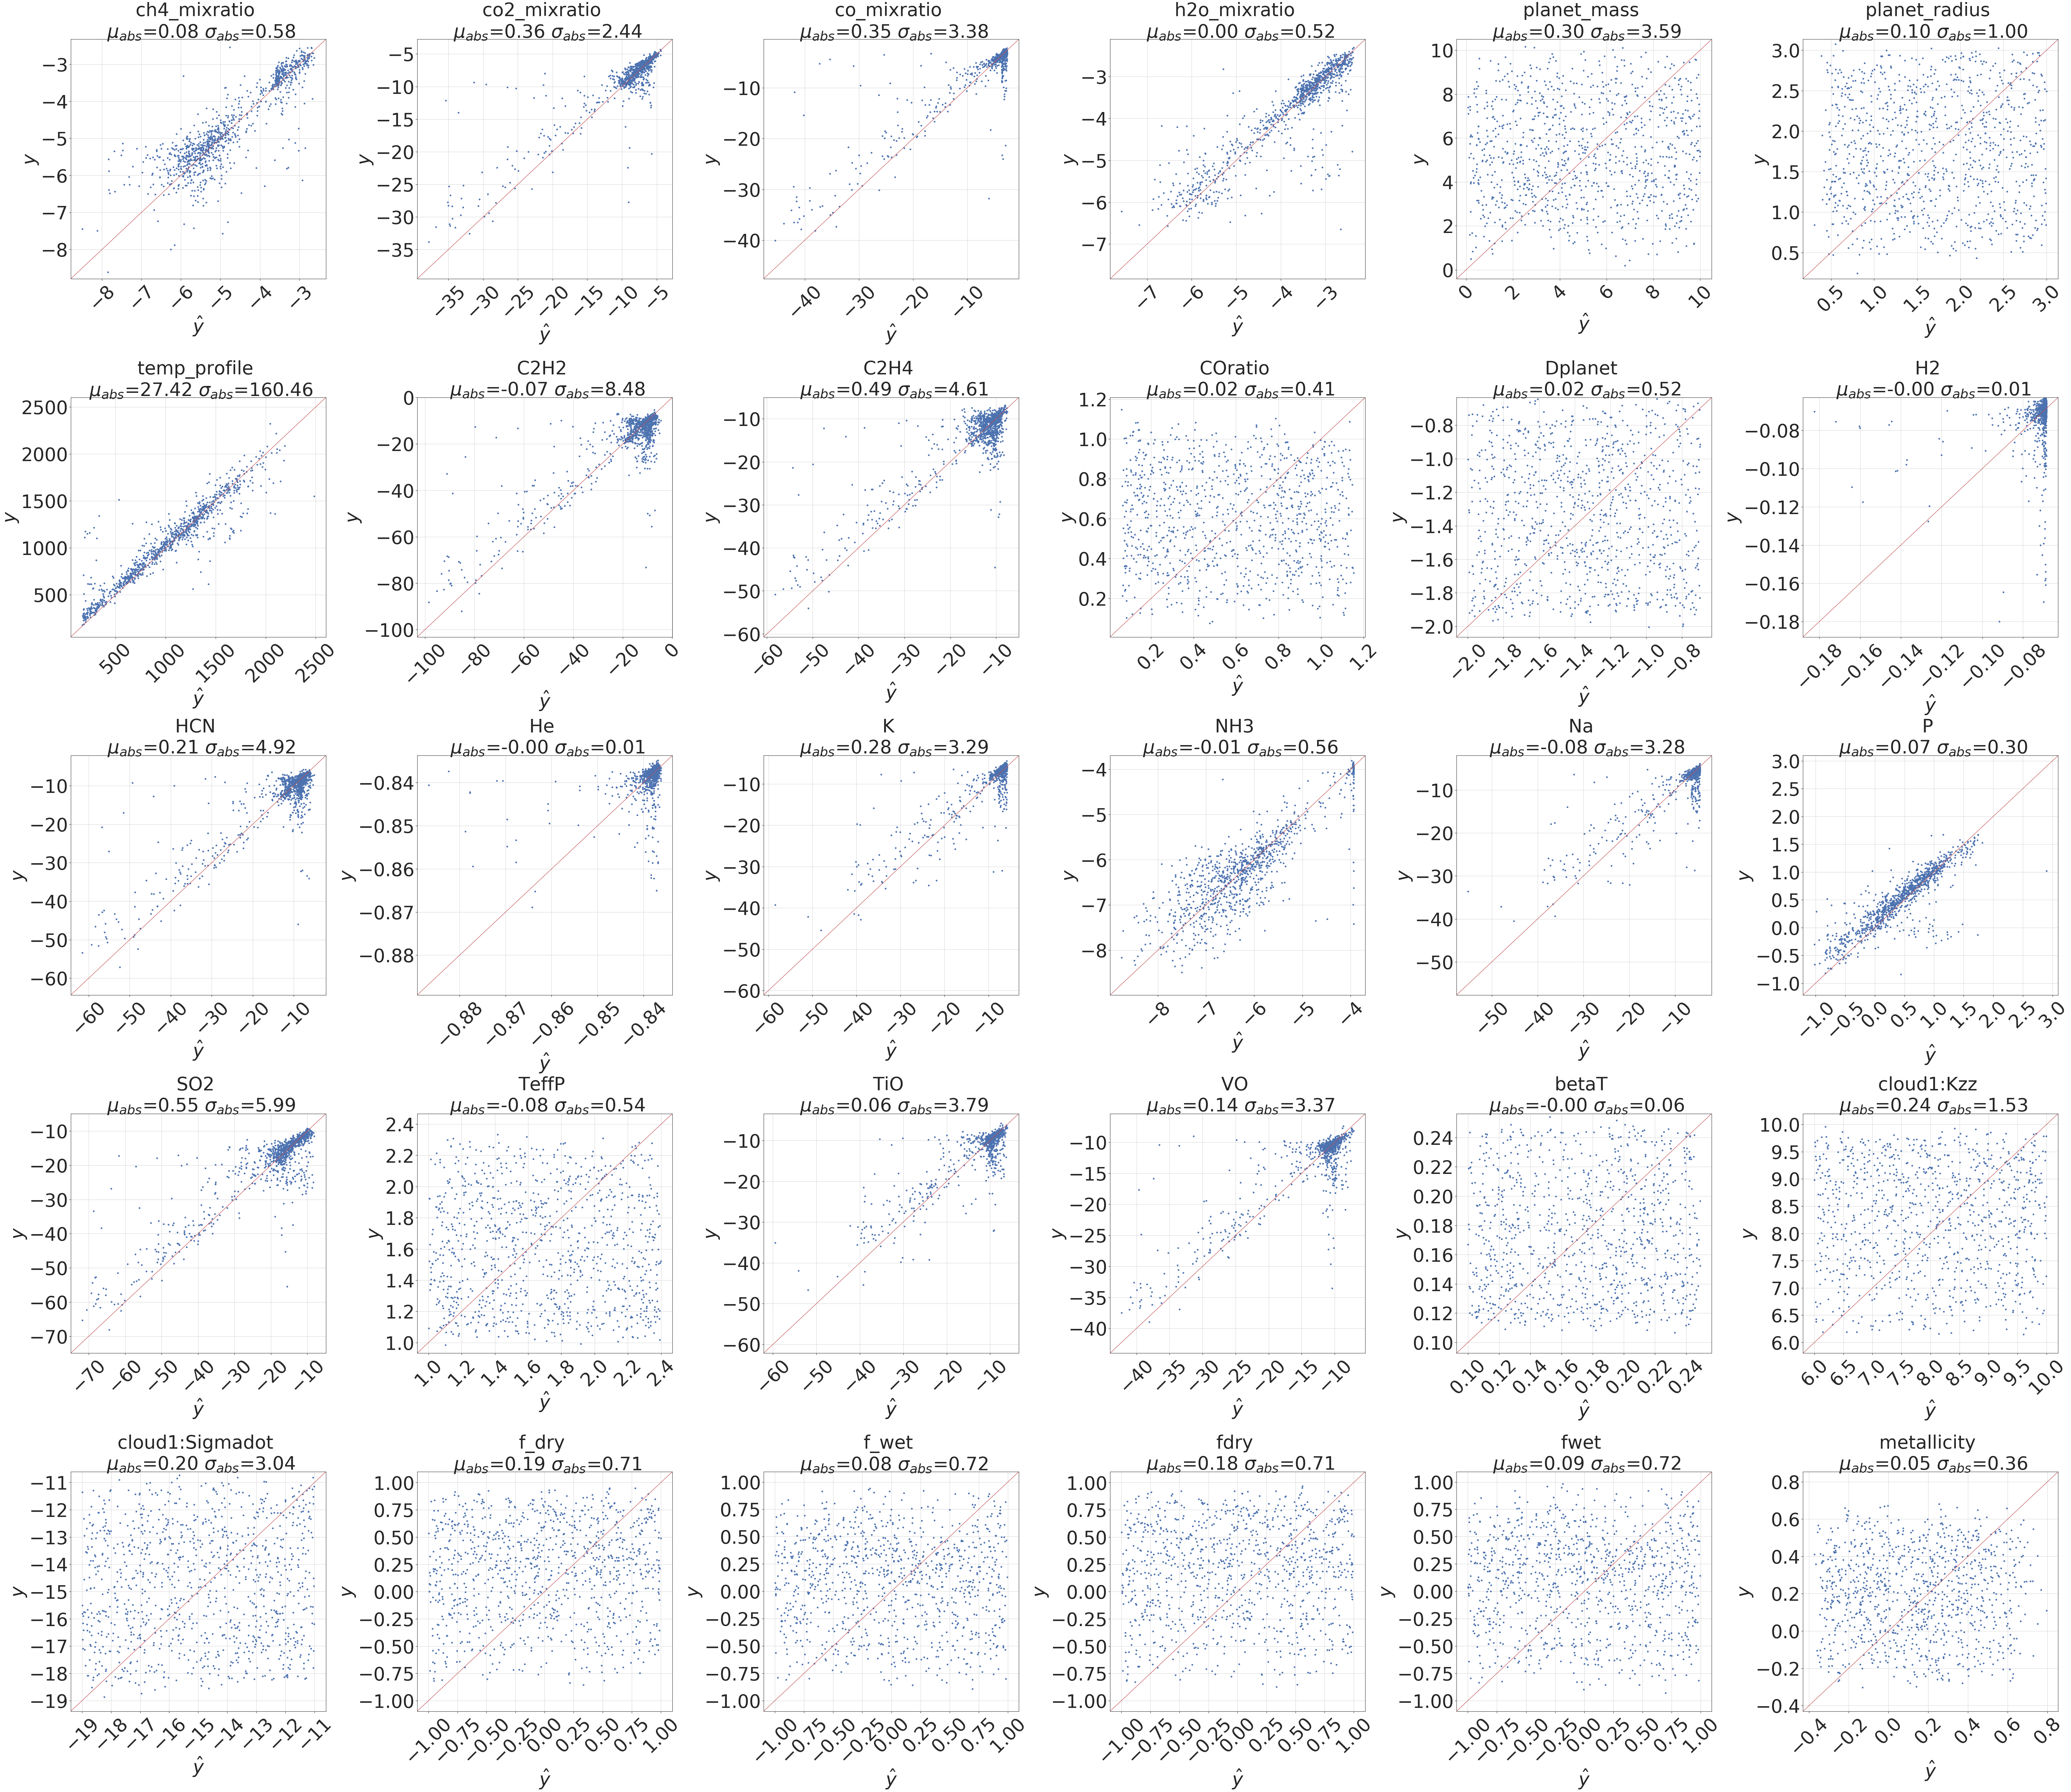
\includegraphics[width=\textwidth,keepaspectratio]{figuren/small gpu2.png}
    \caption{The real versus inpainted values per feature of the complex physical model trained on gpu2, where the red line describes the perfect predictions. This is a sample of 1000 ASPAs from the test set.}
    \label{fig:gan_results_small_gpu2}
\end{figure}

\begin{figure} [!htb]
    \centering
    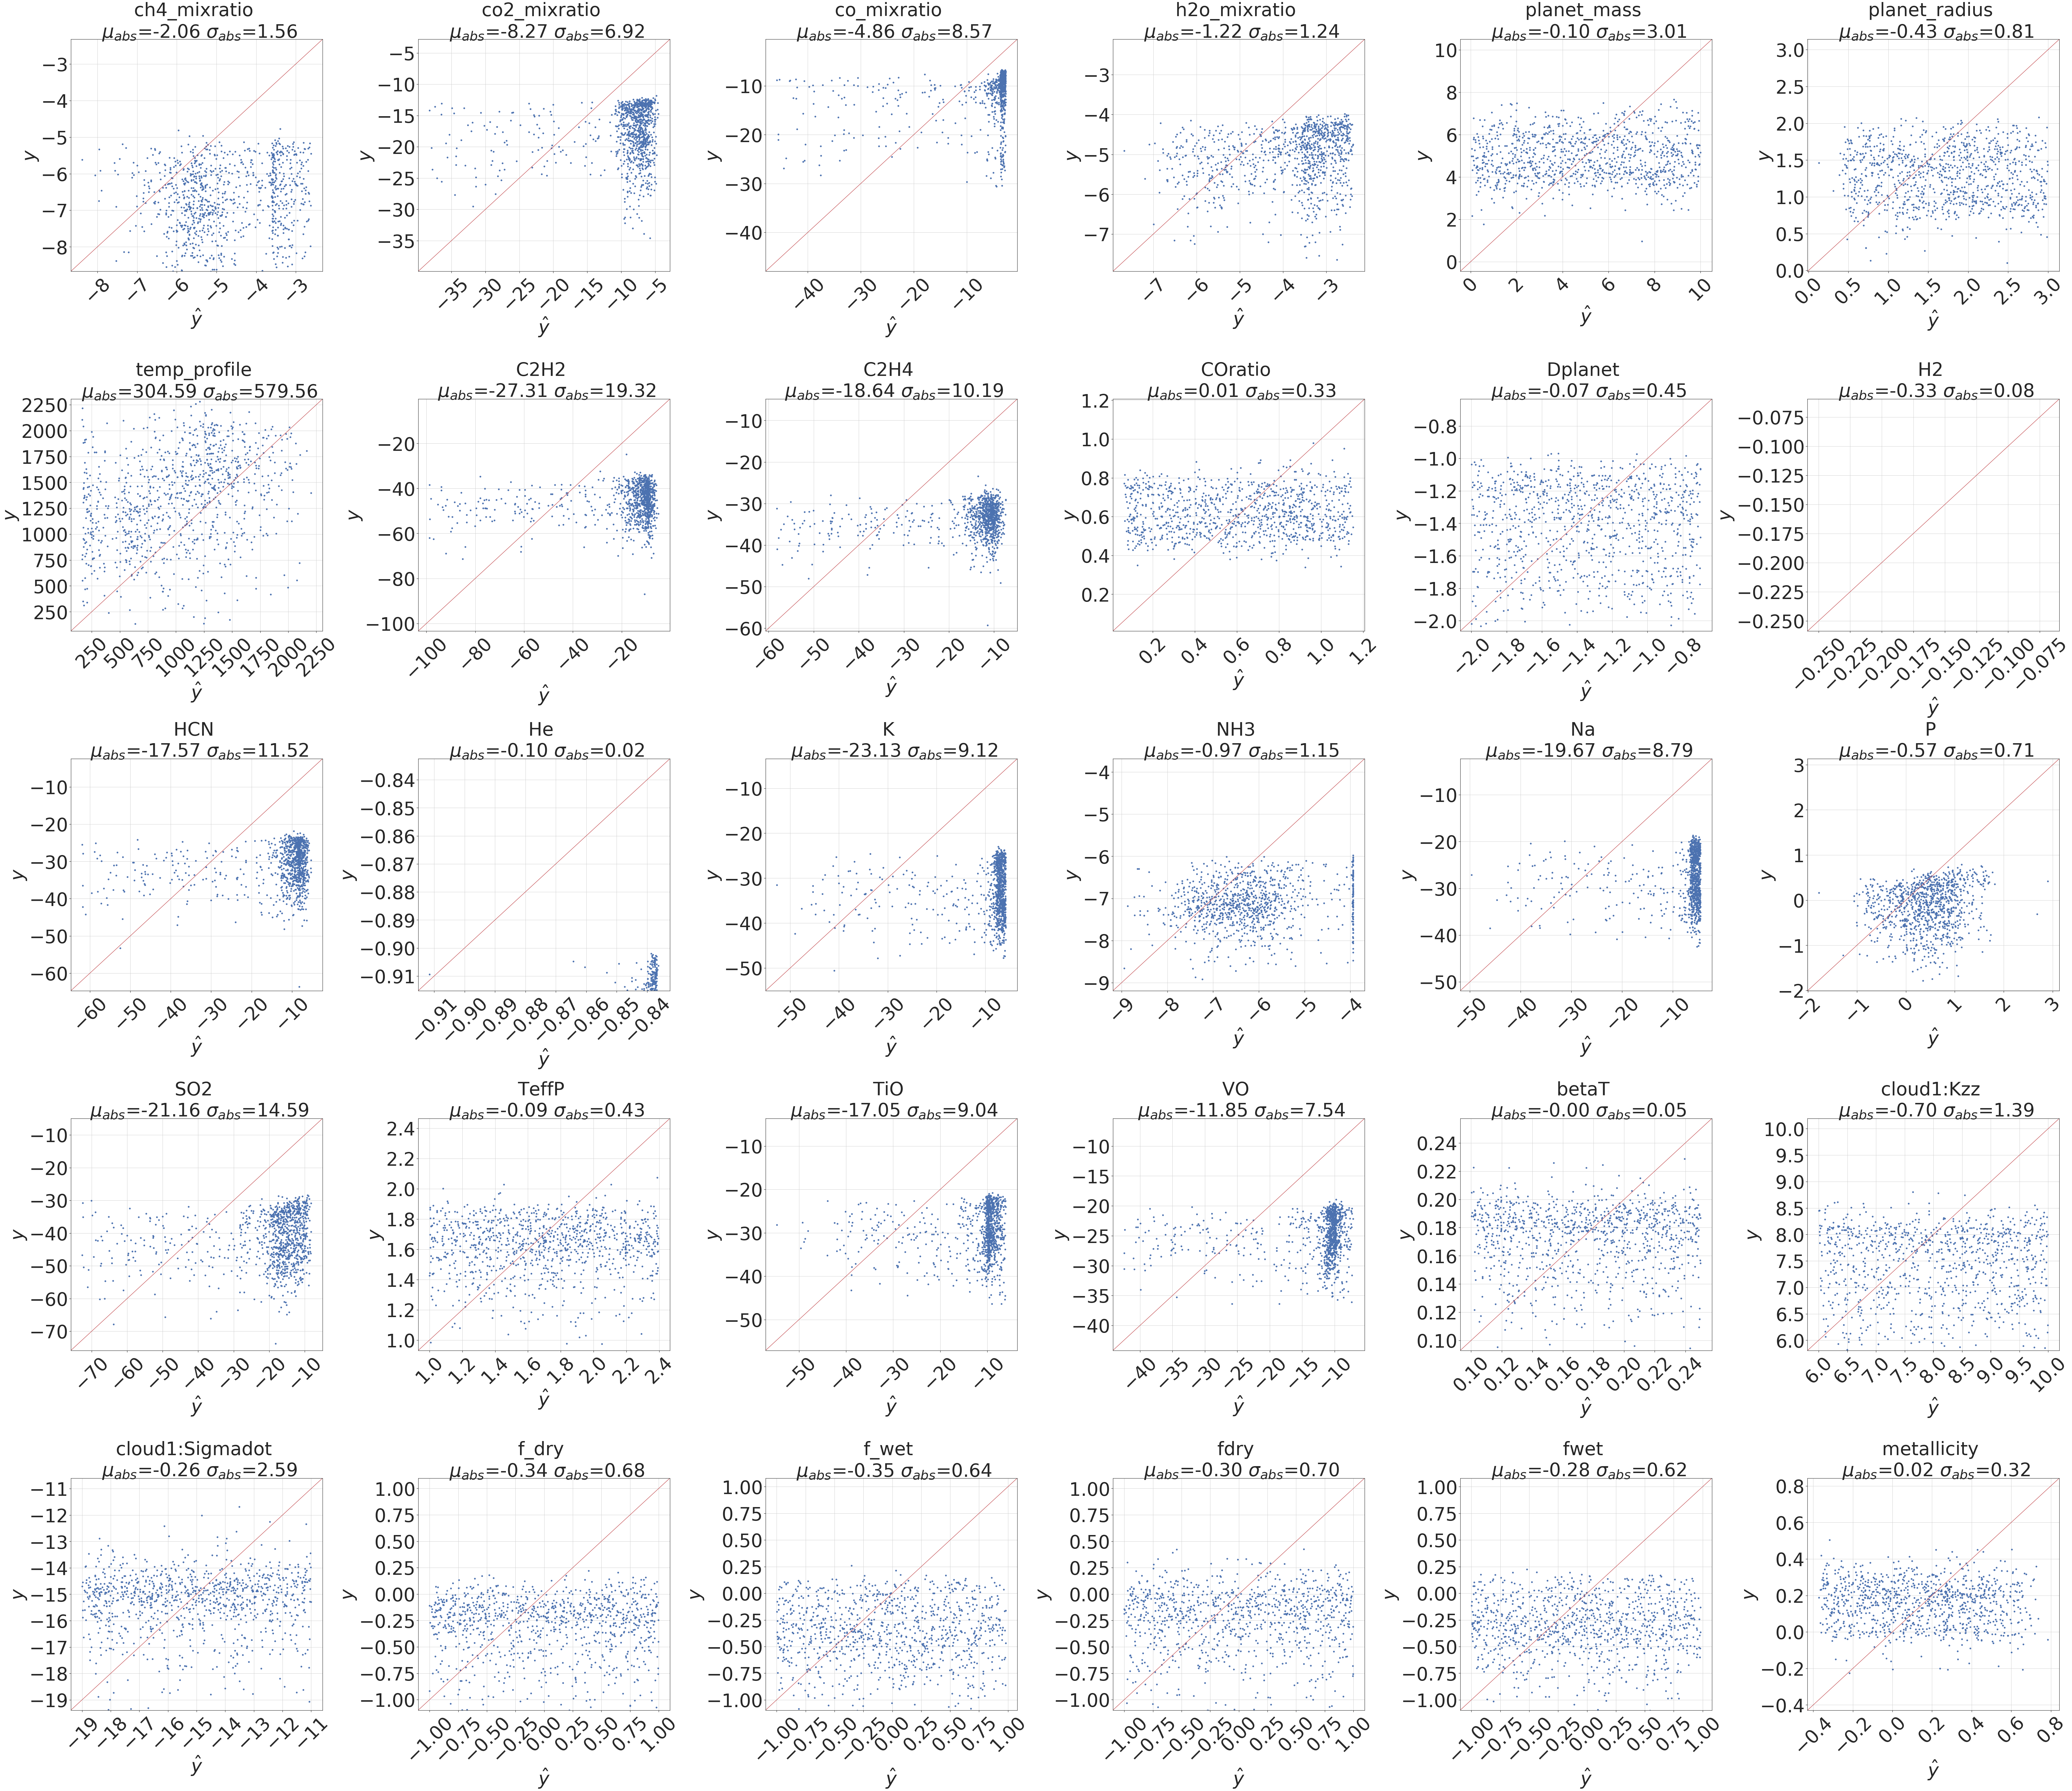
\includegraphics[width=\textwidth,keepaspectratio]{figuren/small gpu3.png}
    \caption{The real versus inpainted values per feature of the complex physical model trained on gpu3, where the red line describes the perfect predictions. This is a sample of 1000 ASPAs from the test set.}
    \label{fig:gan_results_small_gpu3}
\end{figure}

\begin{figure} [!htb]
    \centering
    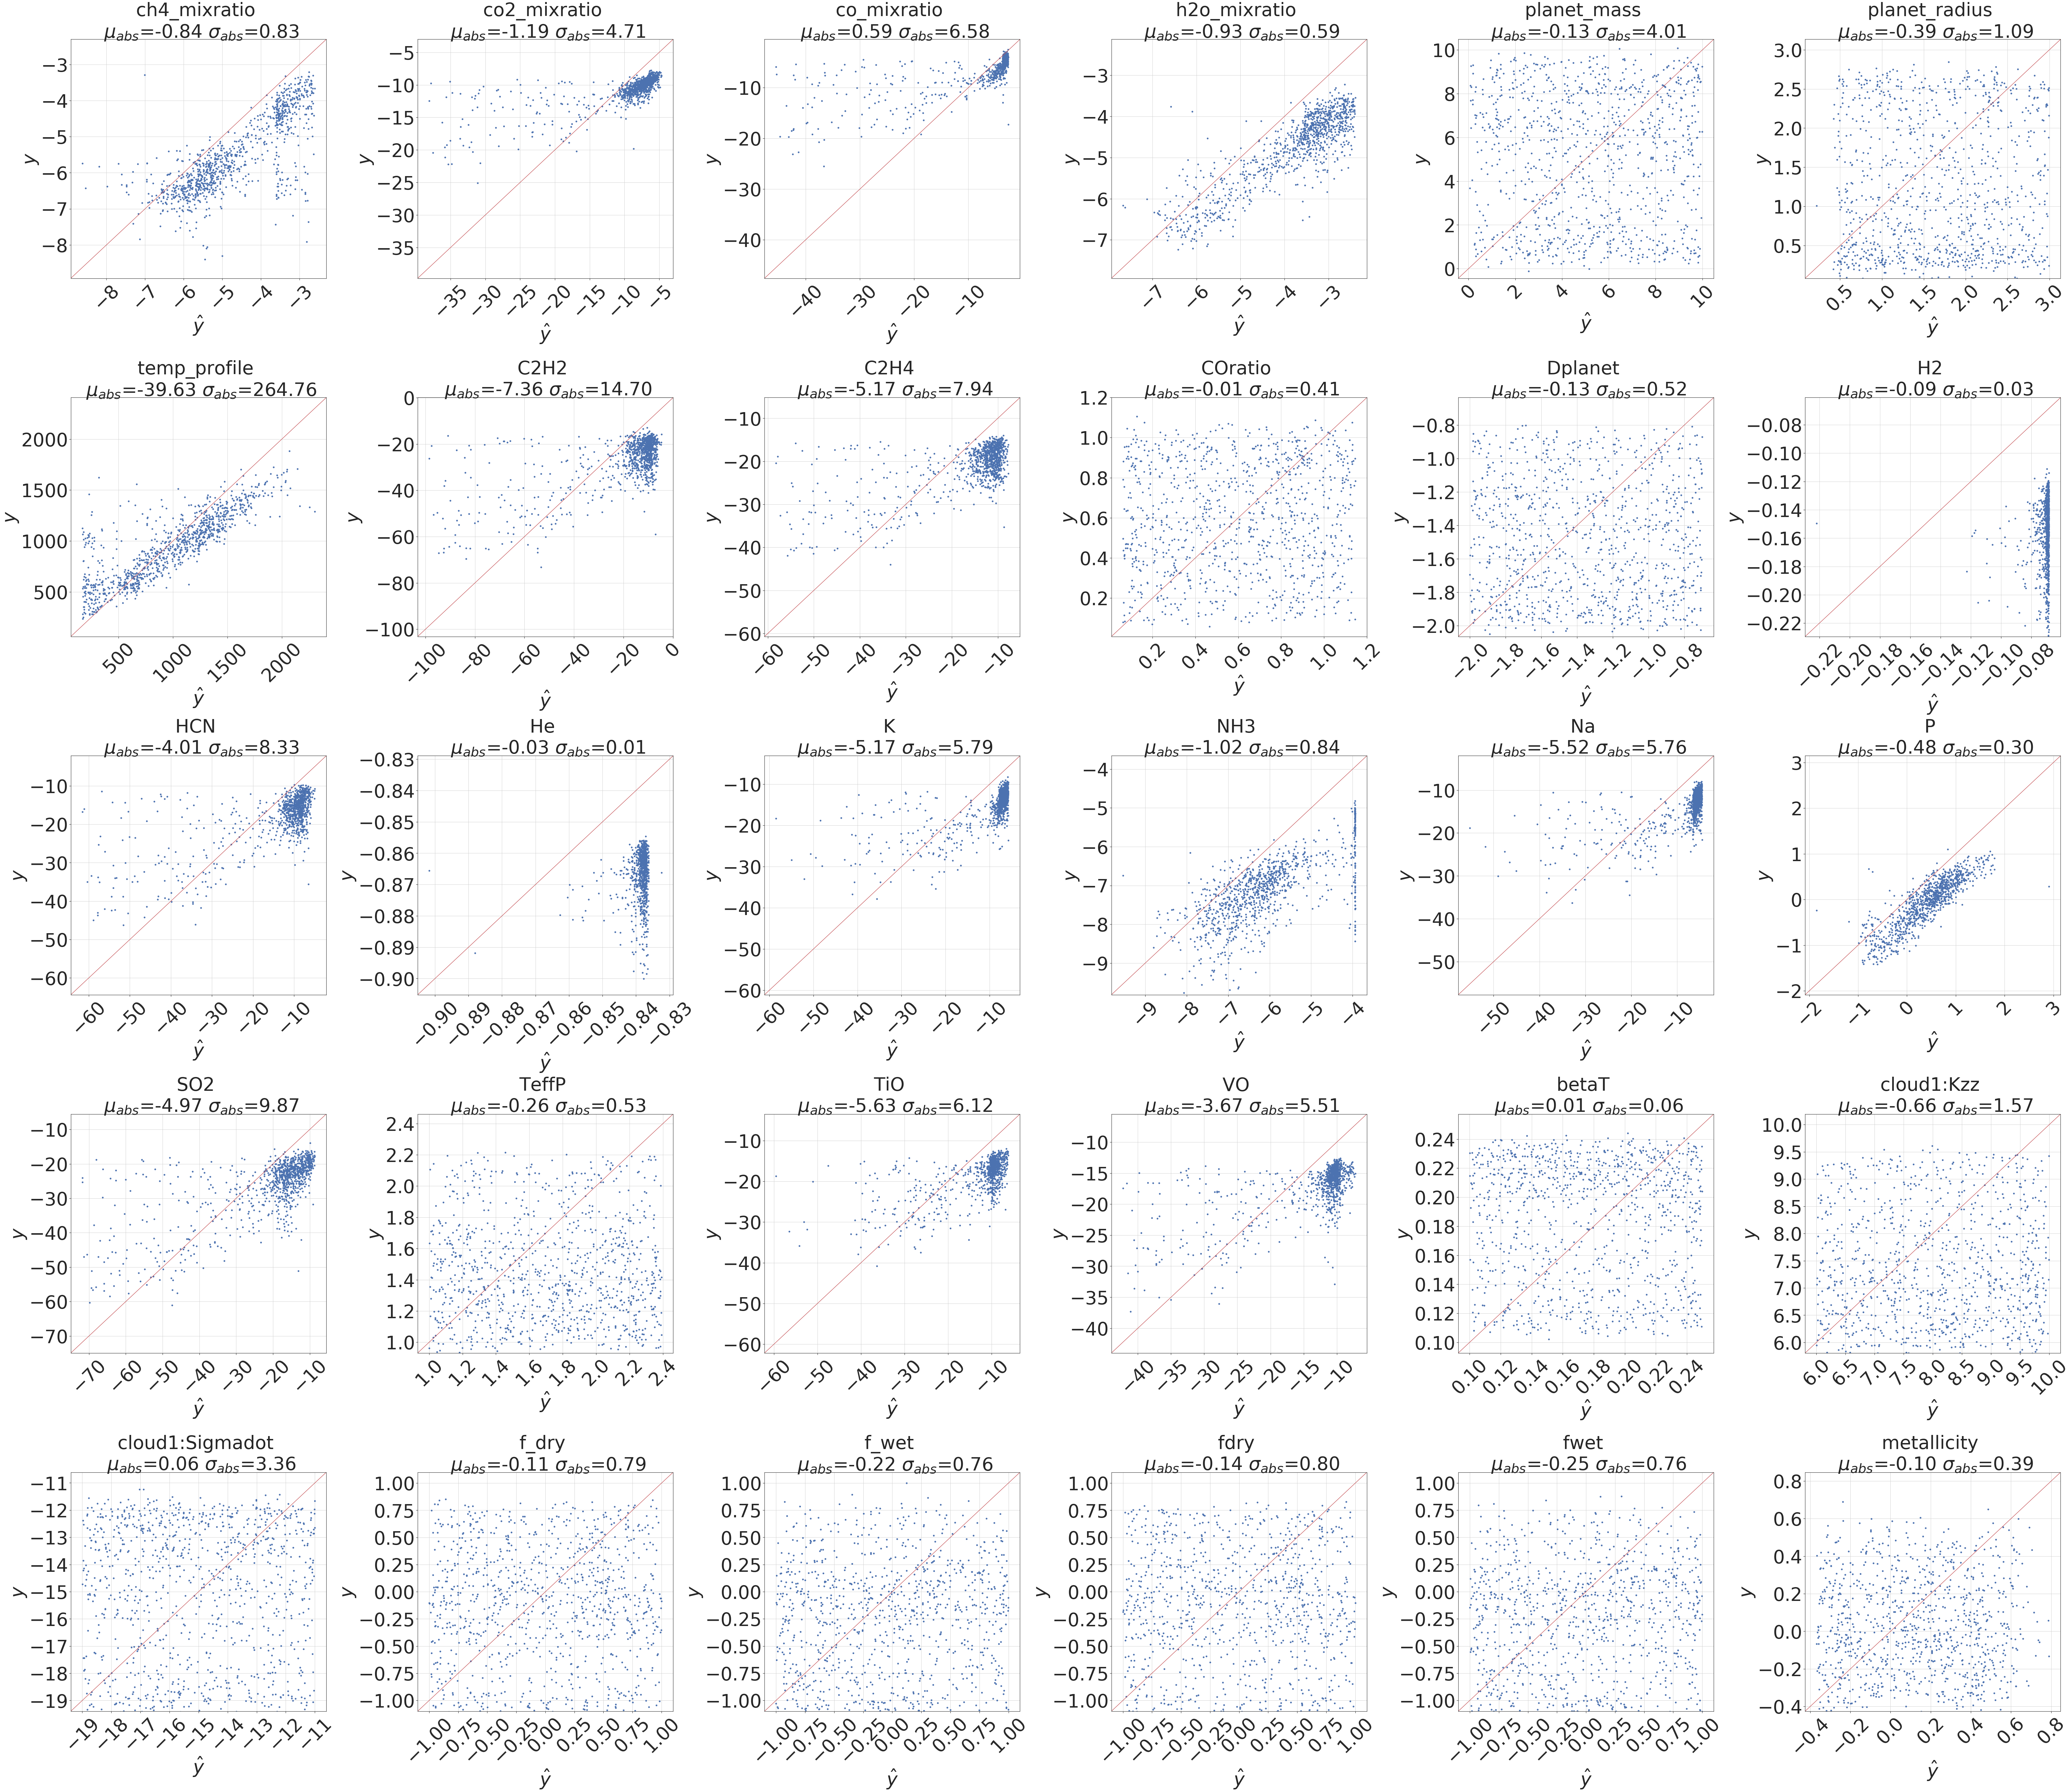
\includegraphics[width=\textwidth,keepaspectratio]{figuren/small gpu4.png}
    \caption{The real versus inpainted values per feature of the complex physical model trained on gpu4, where the red line describes the perfect predictions. This is a sample of 1000 ASPAs from the test set.}
    \label{fig:gan_results_small_gpu4}
\end{figure}

\begin{figure} [!htb]
    \centering
    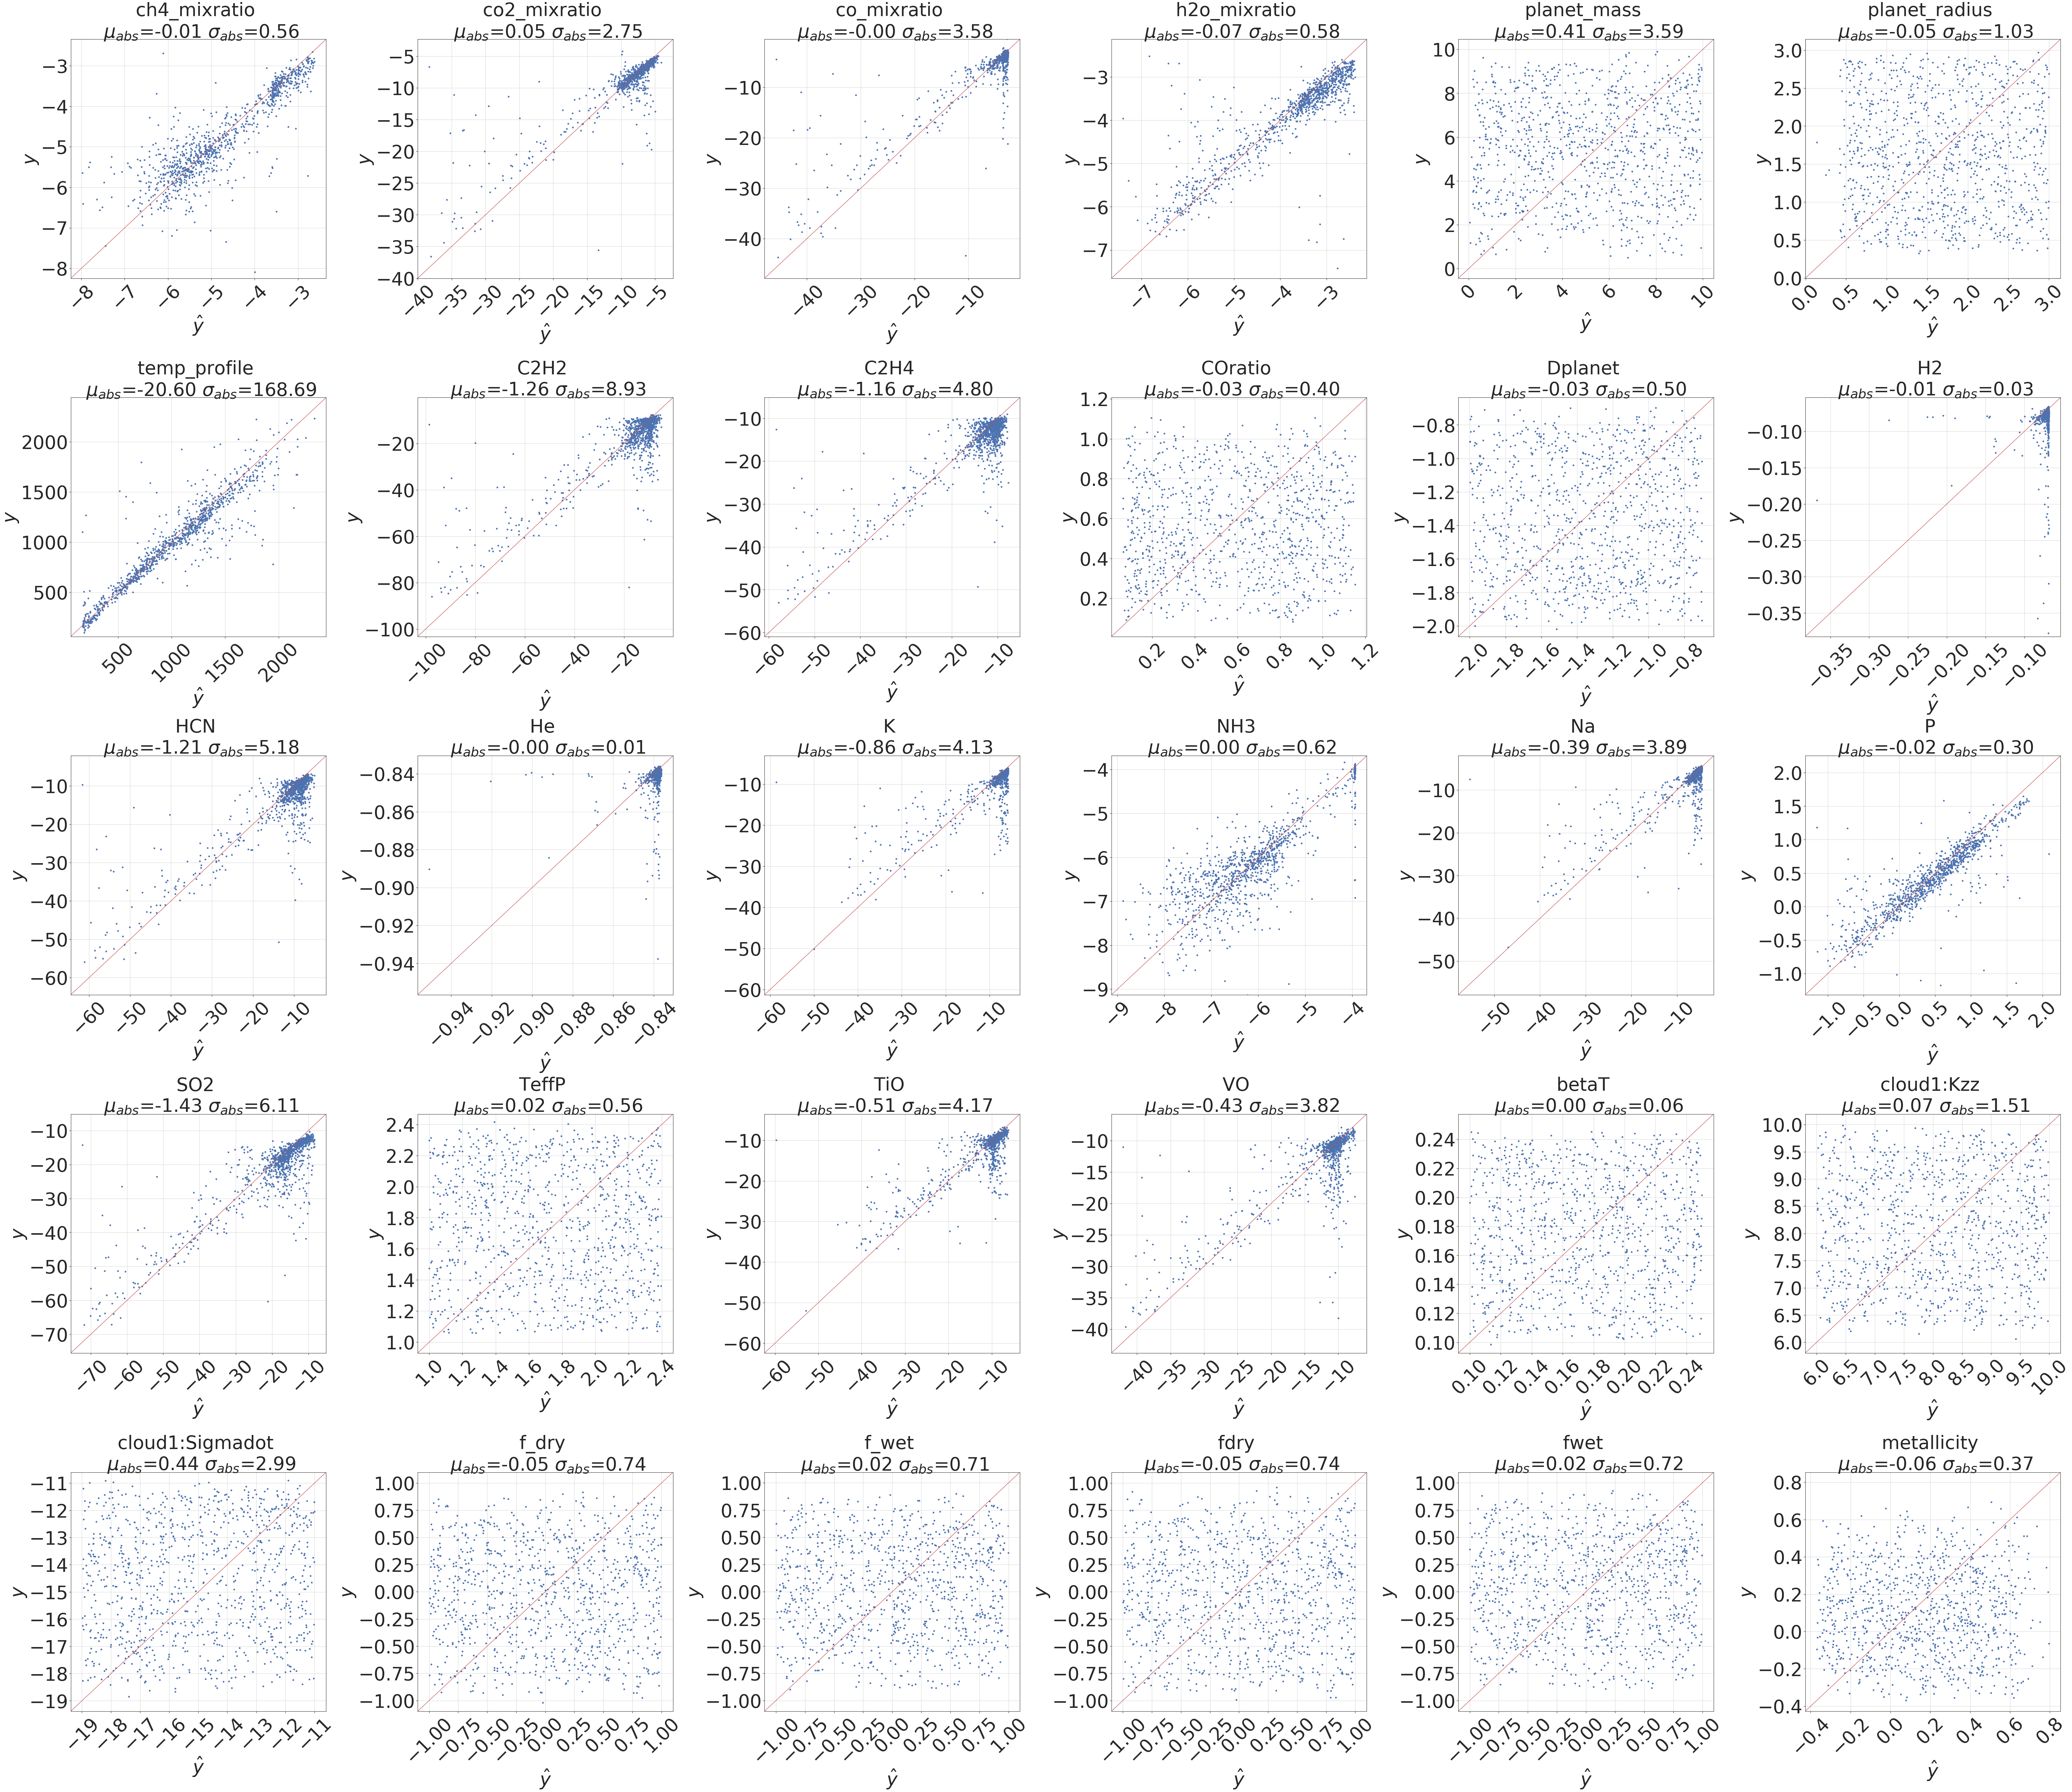
\includegraphics[width=\textwidth,keepaspectratio]{figuren/small gpu5.png}
    \caption{The real versus inpainted values per feature of the complex physical model trained on gpu5, where the red line describes the perfect predictions. This is a sample of 1000 ASPAs from the test set.}
    \label{fig:gan_results_small_gpu5}
\end{figure}